Гравитационное линзирование -- явление отклонения траектории света от прямолинейной в гравитационном поле массивных объектов.  Это достаточно хорошо изученное и подробно описанное в литературе явление (см., например, \cite{gravlensbook}) является, в том числе, одним из независимых способов измерения ряда космологических констант, в частности, постоянной Хаббла $H_0$. 

\subsection{Измерение расстояний в астрономии}

Различные определения расстояния, используемые в космологии, приведены, например, в \cite{distance_measures}. Здесь и далее для описания расстояний между объектами в системе источник -- линза -- наблюдатель используется понятие \textbf{расстояния углового диаметра} (angular diameter distance). Оно определяется по следующей формуле (см, напр., уравн. №№14,15 в \cite{distance_measures}):

\begin{equation}\label{ang_dia_dist}
D_{A}\left(z_{1}, z_{2}\right)=\frac{c}{1+z_{2}} \int_{z_{1}}^{z_{2}} \frac{d z}{H_{0} \sqrt{\Omega_{m}\left(1+z^{3}\right)+\Omega_{\Lambda}}},
\end{equation}
где $H_0=70$ (км/с)/МПк, $\Omega_m=0.3, \Omega_\Lambda=0.7$.

\subsection{Типичная гравитационно-линзированная система}

\begin{equation}\label{sigmacrit}
\Sigma_{crit}=\frac{c^{2}}{4 \pi G} \frac{D_{\mathrm{s}}}{D_{\mathrm{d}} D_{\mathrm{ds}}}
\end{equation}

\begin{equation}\label{convergence}
\kappa = \frac{\Sigma}{\Sigma_{crit}}
\end{equation}

Типичная гравитационно-линзированная система изображена на Рисунке \ref{fig:gravlensfig}. Предполагается, что масса, вызывающая отклонение света, распределена в \textbf{плоскости линзы}. Почти всегда это приближение оправдано, так как характерные размеры самого большого объекта, который может быть линзой, - скопления галактик - порядка 1 МПк, в то время как расстояние между объектами системы порядка 100-1000 МПк. Положения источника света и его изображения задаются углами, отсчитываемыми от оптической оси - линии, проведённой от наблюдателя перпендикулярно плоскости линзы.

\begin{figure}[H]
    \centering
	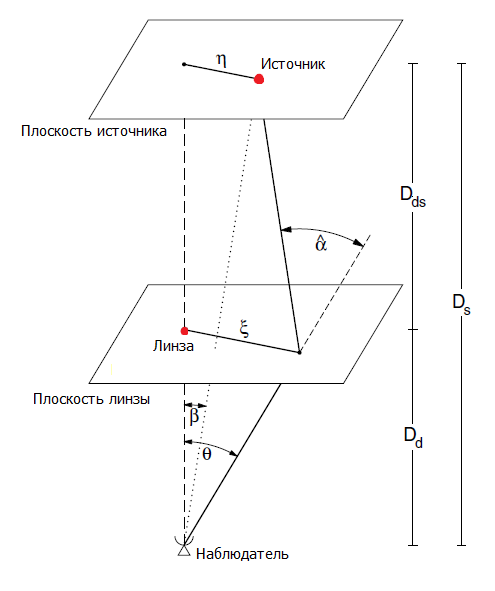
\includegraphics[scale=0.7]{pics/gravlenssyst.png}
	\caption{Типичная гравитационно-линзированная система (\cite{gravlensbook}). Здесь $\beta$ и $\theta$ - углы между оптической осью (пунктирная линия) и источником и его изображением соответственно, $\hat{\alpha}$ - угол отклонения светового луча, $\eta$ и $\xi$ - расстояния от оптической оси до источника и его изображения соответственно,  $D_d$ - расстояние между наблюдателем и плоскостью линзы, $D_{ds}$ - между плоскостями линзы и источника, $D_s$ - между наблюдателем и источником.\label{fig:gravlensfig} }
   \end{figure} 



Для дальнейшего описания гравитационного линзирования необходимо ввести величину, описывающую характерное поперечное расстояние в рассматриваемой системе. Таким расстоянием (угловым) является радиус Эйнштейна

\begin{equation}\label{r_ein}
\theta_{E}=\sqrt{\frac{4 G M}{c^{2}} \frac{D_{d s}}{D_{d} D_{s}}}
\end{equation}

где $M$ - масса линзы, $c$ - скорость света, $G$ - гравитационная постоянная, $D_d$, $D_s$ и $D_{ds}$ - расстояния (расстояния углового диаметра) от наблюдателя до плоскости линзы, до источника и между плоскостями линзы и источника соответственно (см. Рис. \ref{fig:gravlensfig}).

\subsection{Усиление и искажение изображений}

С точки зрения линейной алгебры, гравитационное линзирование - это отображение одной плоскости на другую, которое задаётся следующей матрицей:

\begin{equation}
\mathcal{A}(\boldsymbol{\theta})=\frac{\partial \boldsymbol{\beta}}{\partial \boldsymbol{\theta}}=\left(\delta_{i j}-\frac{\partial^{2} \psi(\boldsymbol{\theta})}{\partial \theta_{i} \partial \theta_{j}}\right)=\left(\begin{array}{cc}{1-\kappa-\gamma_{1}} & {-\gamma_{2}} \\ {-\gamma_{2}} & {1-\kappa+\gamma_{1}}\end{array}\right)
\end{equation}

В ней есть две основные составляющие: конвергенция, отвечающая за изменение линейных размеров изображения (увеличение или уменьшение), и двухкомпонентный сдвиг (shear), характеризующий искажение формы изображений. Усиление изображения обратно пропорционально определителю этой матрицы (то есть якобиану этого отображения):

\begin{equation}
\mu=\frac{1}{\operatorname{det} A}
\end{equation}

Видно, что возможно существование некоторого множества точек, в которых усиление формально бесконечно. Кривая, образуемая этими точками, называется каустикой, а её образ в плоскости линзы – критической кривой. На Рисунке 2 видно, как ведёт себя изображение (в плоскости линзы) источника при пересечении им складки (fold) или излома (cusp) каустики.
 
\begin{figure}[h!]
    \centering
	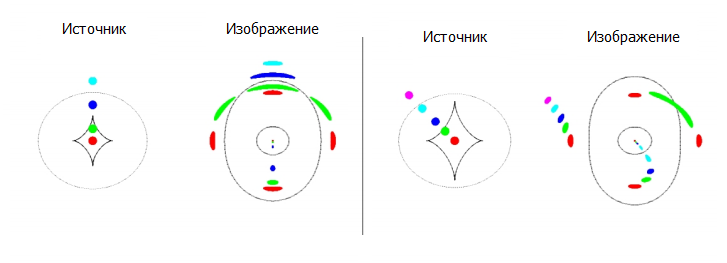
\includegraphics[scale=0.8]{pics/caust_intro.png}
	\caption{Поведение изображения (в плоскости линзы) источника при пересечении им излома(слева) или складки (справа) каустики. Рисунок из \cite{narbart}.}
\end{figure}

\subsection{Появление нескольких изображений}

Важным свойством гравитационного линзирования является возможность появления нескольких изображений одного и того же источника. В присутствии линзы существует дополнительная временная задержка между временем излучения света и моментом его прихода к наблюдателю по сравнению с прямолинейным приходом света:

\begin{equation}
\tau(\boldsymbol{\theta})=\frac{D_{d} D_{s}}{c D_{d s}}\left[\frac{1}{2}(\boldsymbol{\theta}-\boldsymbol{\beta})^{2}-\Psi(\boldsymbol{\theta})\right]
\end{equation}

Здесь первое слагаемое означает геометрическую задержку (удлиняется траектория распространения света), второе - гравитационную (в соответствии с ОТО время около гравитирующих тел идет “медленнее”);  и  - положения (в угловых единицах) соответственно изображения и источника (см. Рис.\ref{fig:gravlensfig}), $\Psi(\boldsymbol{\theta})$ - линзирующий гравитационный потенциал. Так как оба слагаемых пропорциональны $H_0^{-1}$, то, измеряя временную задержку между изображениями одного и того же источника, можно получить значение постоянной Хаббла (см., напр., \cite{refsdal1964}).

\section{Возможные источники}

Для таких измерений блеск источника должен быть переменным. В таком случае, разные изображения, возникающие в результате гравитационного линзирования будут изменять свой блеск также, как и источник, но с некоторой задержкой по времени. В качестве возможных источников для таких измерений используются квазары - они весьма яркие и почти точечные. На текущий момент опубликовано большое количество работ, посвящённых гравитационно линзированным квазарам и измерению при их помощи постоянной Хаббла (см, напр., работу \cite{holicow}, а также ссылки в ней). 

Другим подходящим источником являются сверхновые - их кривые блеска имеют чётко выраженный пик, а наблюдения занимают сравнительно небольшие времена, что значительно упрощает измерения. Впервые идея использовать линзированные сверхновые для оценки постоянной Хаббла была предложена Сьюром Рефсдалом в 1964 году (\cite{refsdal1964}). На текущий момент известны только две гравитационно линзированные сверхновые со множественными изображениями, SN Refsdal (\cite{kelly2014}), названная в честь Сьюра Рефсдала, и SN iPTF16geu (\cite{goobar2017}). Однако с запуском в ближайшее время обсерватории LSST ожидается открытие десятков таких систем (\cite{pierelrodney2019}), что делает задачу разработки алгоритма анализа гравитационно линзированных сверхновых важной и своевременной.